
%\begin{center}
%\LARGE{\textbf{  Installation of Microsoft's Kinect for Windows SDK}}
%\end{center}




\begin{flushleft}

\chapter{Establishing Unicast connection between 2 XBee modules}


\medskip
\section{\textbf{Installation of X-CTU (Windows)}}
\medskip
Hello world ! This is a quick installation tutorial for Digi's X-CTU software.
The X-CTU Software enables you to configure and test various kinds of communication modes between XBee modules.
\medskip
\subsection{\textbf{ System Requirements}}
\medskip
\textbf{Supported Operating Systems}
Windows 98, ME, 2K, XP, Vista, 7, 8, 8.1
\medskip
\textbf{Non-supported Operating Systems}
Windows 95, NT, Unix, Linux
\medskip
\textbf{Hardware Requirements}
\medskip
\begin{itemize}
\item 2 XBee modules
\item 1 XBee USB adapter 
\item Dedicated USB 2.0 bus
\item USB A-Type Male to USB B-Type Male Cable
\item Firebird V robot
\end{itemize}
\medskip

\subsection{\textbf{ Installation Procedure}}
\textbf{Step 1 :}

\medskip


\begin{figure}
\begin{center}
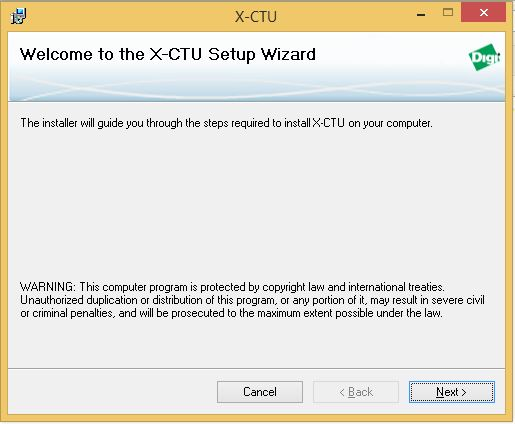
\includegraphics[scale=0.5]{zigbee_1}
\textbf{\caption{Step 1 - Welcome to X-CTU Setup Wizard}}
\end{center}
\end{figure}
\medskip

Launch Setup\_XCTU\_5260.exe to start installation of Digi's X-CTU software for configuration of XBee modules. Click "Next" to continue. Shown in figure 2.1. 
\medskip
\textbf{Step 2 :}

\medskip

\begin{figure}
\begin{center}
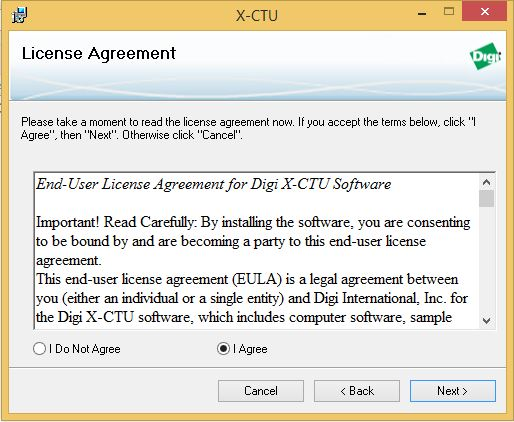
\includegraphics[scale=0.5]{zigbee_2}
\textbf{\caption{Step 2 - License Agreement}}
\end{center}
\end{figure}
\medskip

Read the license agreement and select the "I Agree" radio button if you wish to continue.Click "Next".
Shown in figure 2.2.

\medskip

\textbf{Step 3 :}

\medskip

\begin{figure}
\begin{center}
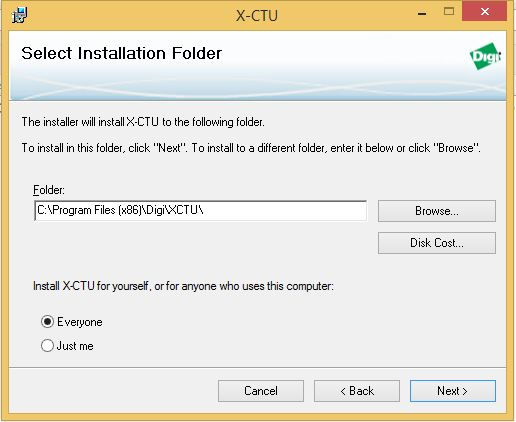
\includegraphics[scale=0.5]{zigbee_3}
\textbf{\caption{Step 3 - Select Installation Folder}}
\end{center}
\end{figure}
\medskip

Select the installation folder you wish to install X-CTU to, and whether you wish to install for Everyone or just the current user.Click "Next".
Shown in figure 2.3.

\medskip

\textbf{Step 4 :}

\medskip

\begin{figure}
\begin{center}
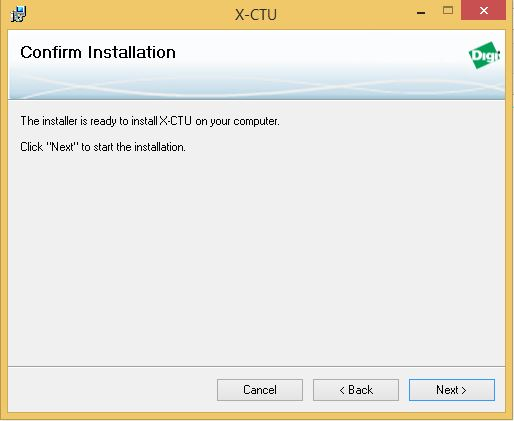
\includegraphics[scale=0.5]{zigbee_4}
\textbf{\caption{Step 4 - Confirm Installation}}
\end{center}
\end{figure}
\medskip

Confirm the installation by clicking "Next".Shown in figure 2.4.

\medskip

\textbf{Step 5 :}

\medskip

\begin{figure}
\begin{center}
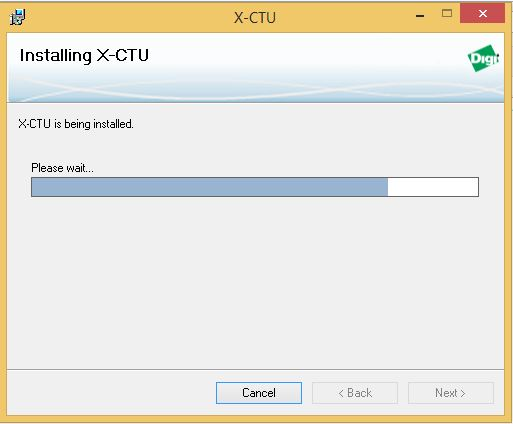
\includegraphics[scale=0.5]{zigbee_5}
\textbf{\caption{Step 5 - Installing X-CTU}}
\end{center}
\end{figure}
\medskip

Wait till the installation is complete.
If you wish to check out Digi's website for firmware updates, click "Yes", else click "No". Shown in figure 2.5.
 
\medskip

Congratulations! X-CTU was successfully installed if you followed the above steps correctly. Click "Close" to close the installation window.

\medskip
\subsection{\textbf{ Configuring 2 XBee modules for unicast connection}}
\medskip
Hello world ! This is a quick tutorial for configuration of 2 XBee modules for working in Unicast mode.

\textbf{Step 1 :}

\medskip

\begin{figure}
\begin{center}
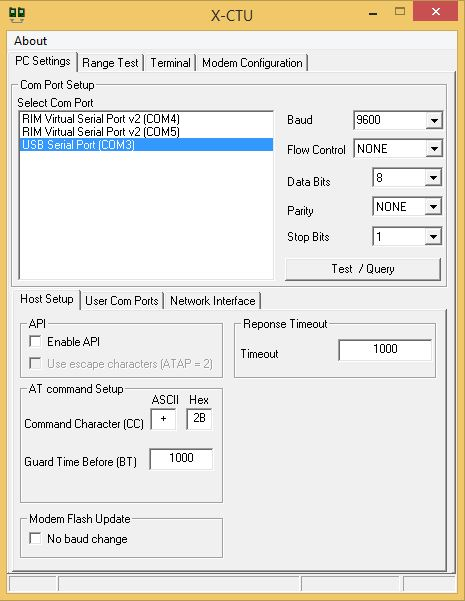
\includegraphics[scale=0.5]{zigbee_8}
\textbf{\caption{Step 1 - X-CTU User Interface}}
\end{center}
\end{figure}
\medskip

\begin{figure}
\begin{center}
\includegraphics[scale=0.1]{zigbee_17}
\textbf{\caption{Step 1 - Connecting XBee module with XBee USB adapter}}
\end{center}
\end{figure}
\medskip


Plug in an XBee module in the XBee USB adapter and connect it to a USB port of the PC. Launch X-CTU. Select the "USB Serial Port(COM3)" entry under the "Select Com Port" title. The COM port number varies according to hardware configuration. It might be different for you. Setup the COM port according to the settings shown in the figure. Shown in figures 2.6 and 2.7.

\medskip

\textbf{Step 2 :}

\medskip
\begin{figure}
\begin{center}
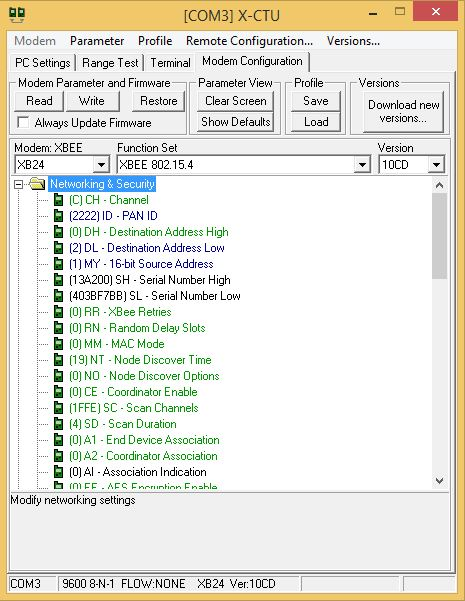
\includegraphics[scale=0.5]{zigbee_11}
\textbf{\caption{Step 2 - Reading the Modem Parameters}}
\end{center}
\end{figure}
\medskip

Go to the "Modem Configuration" tab and click "Read" under "Modem Parameter and Firmware" section. The Modem Parameters will appear in the viewing area below. If they don't appear and such a pop-up comes up, press the "Reset" button on the Zigbee USB adapter and try reconnecting the adapter and then pressing the "Reset" button if it does not work.
Shown in figure 2.8.

\medskip
\textbf{Step 3 :}

\medskip
\begin{figure}
\begin{center}
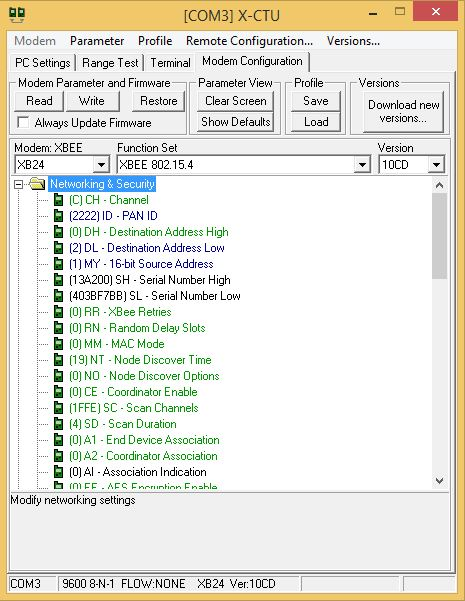
\includegraphics[scale=0.5]{zigbee_11}
\textbf{\caption{Step 3 - Configuring the Modem parameters for XBee module 1}}
\end{center}
\end{figure}
\medskip

\begin{figure}
\begin{center}
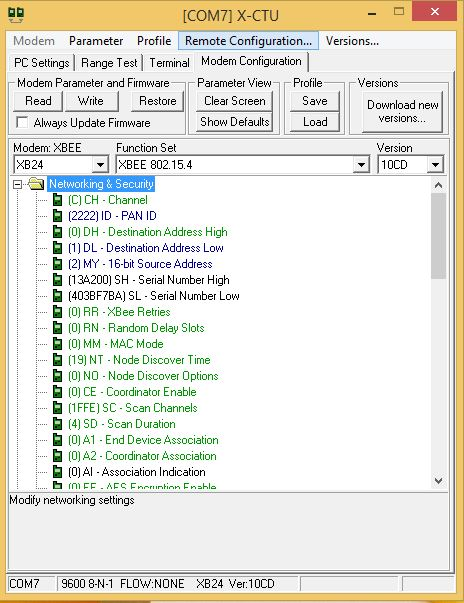
\includegraphics[scale=0.5]{zigbee_13}
\textbf{\caption{Step 3 - Configuring the Modem parameters for XBee module 2}}
\end{center}
\end{figure}
\medskip

The parameters for both the XBee modules have to be set. Set the Channel and PAN ID of both the XBee modules as same. Set Destination Address High(DH) for both the modules as 0. The Destination Address Low(DL) and 16-bit Source Address(MY) have to be set such that the DL of one module is the MY of the other and MY of one module is the DL of other for both the modules. Here DL=2, MY=1 was used for the first module, and vice-versa for the other as shown in the figure.
 Configuration of the 2 Zigbee modules can be done one after another or simultaneously by launching 2 instances of X-CTU and connecting both the modules with the PC. Following these steps will configure the X-Bee modules in unicast mode, i.e. simple one-to-one wireless communication. It is recommended not to change the rest of the parameters and leave them at their default values. However, if you are an advanced user, you may tinker with their values if you know what you are doing.
Shown in figures 2.9 and 2.10 for both the modules.

\medskip
\textbf{Step 5 :}

\medskip
\begin{figure}
\begin{center}
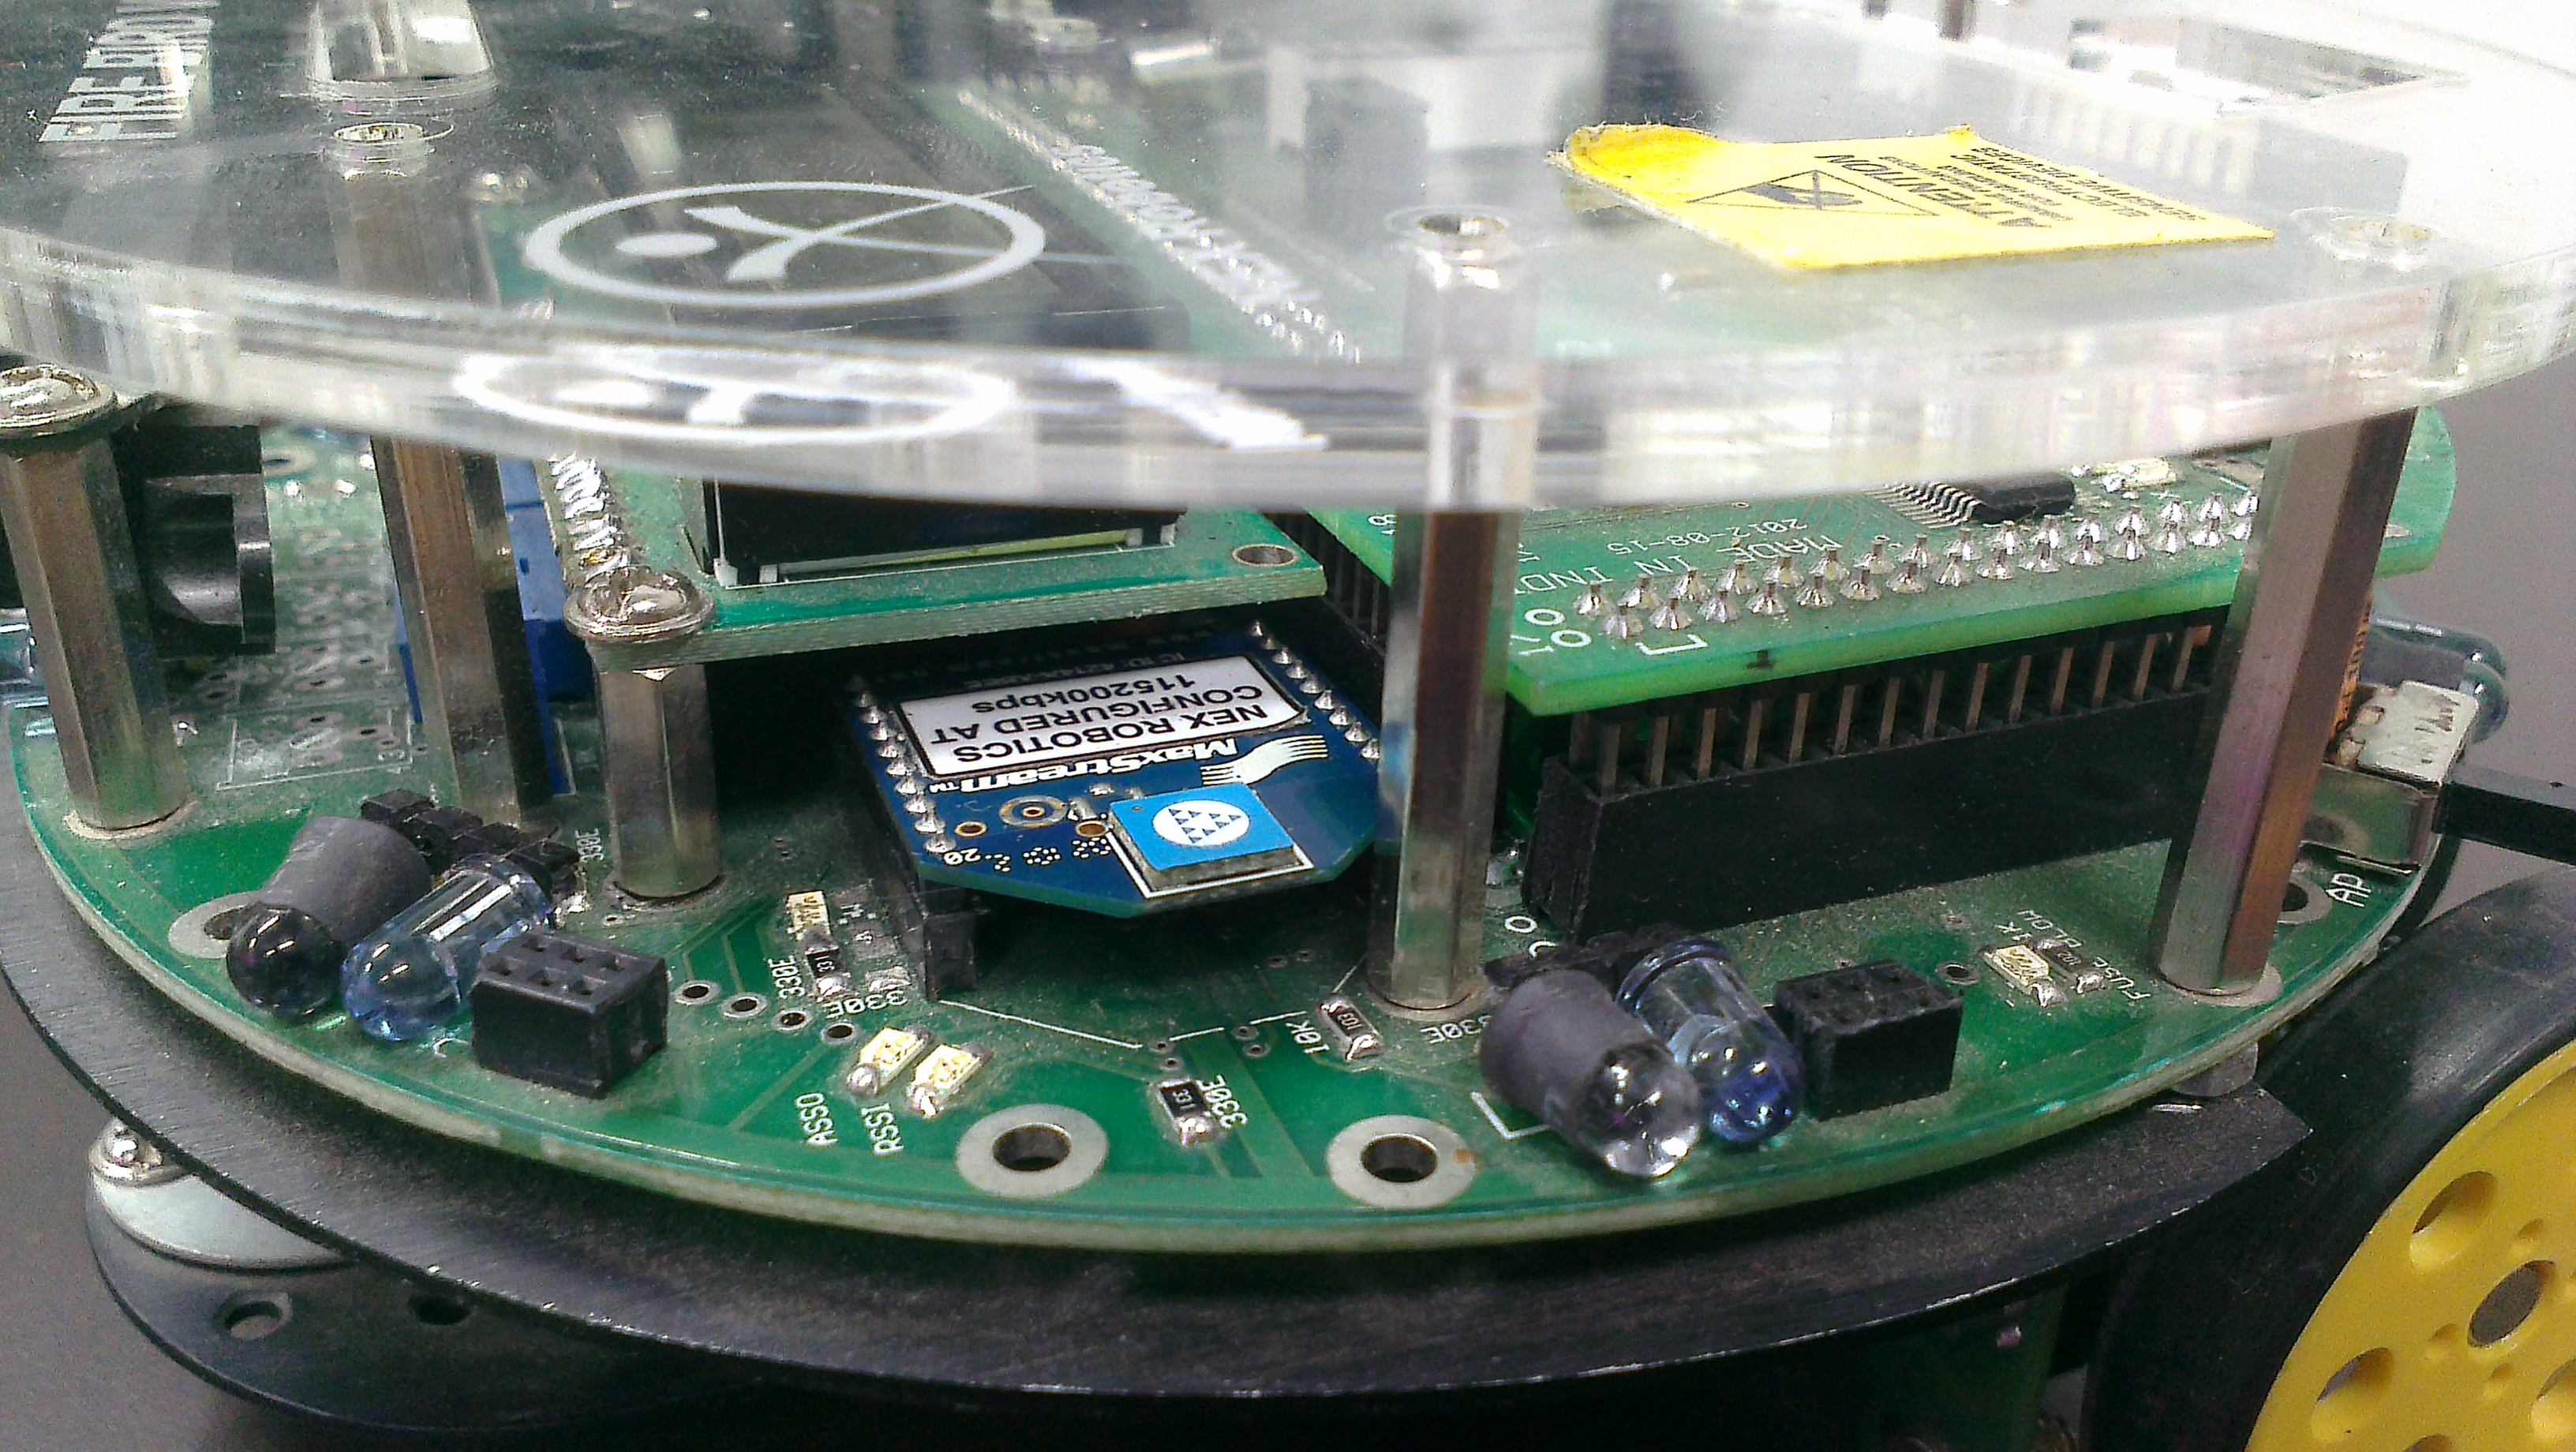
\includegraphics[scale=0.1]{zigbee_16}
\textbf{\caption{Step 4 - Connecting Zigbee module to Firebird V}}
\end{center}
\end{figure}
\medskip


\medskip
\begin{figure}
\begin{center}
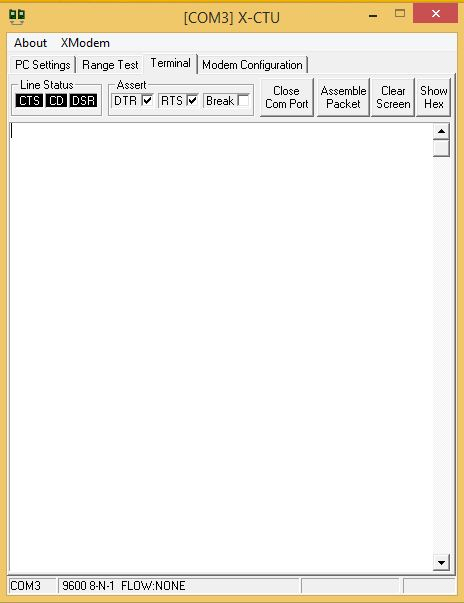
\includegraphics[scale=0.5]{zigbee_14}
\textbf{\caption{Step 4 - X-CTU's terminal Wizard}}
\end{center}
\end{figure}
\medskip

After configuration of both the XBee modules, leave one of the modules in the USB Adapter and plug the other one in the Firebird V robot's X-Bee slot. Load the program "\_Interfacing\_Kinect\_To\_Firebird\_Using\_Zigbee.hex" provided with this document on the Firebird V robot. Start the X-CTU software and go to the "Terminal" tab.  You can send these byte sized commands to the Firebird V robot to test the wireless connection via XBee: 

\begin{tabular}{|c|c|c|}
\hline Keyboard Key & ASCII Value & Action \\ 
\hline 8 &  0x38 & Forward \\ 
\hline 2 &  0x32 & Backward \\ 
\hline 4 &  0x34 & Left \\ 
\hline 6 &  0x36 & Right \\ 
\hline 5 &  0x35 & Stop \\ 
\hline 7 &  0x37 & Buzzer On \\ 
\hline 9 &  0x39 & Buzzer Off \\ 
\hline 
\end{tabular}
\bigskip

\textbf{\Large{Congratulations!  you just established a unicast connection between 2 X-Bee modules. Shown in figure 2.11 and 2.12.}}


\end{flushleft}

